% NERACA: groundwater accounts, inspection leads and pipes -- research report and app design
% Compile: pdflatex main.tex (twice)
\documentclass[11pt,a4paper]{article}
\usepackage[T1]{fontenc}
\usepackage[utf8]{inputenc}
\usepackage[sc]{mathpazo}
\usepackage[scaled=0.92]{helvet}
\renewcommand{\ttdefault}{lmtt}
\usepackage{microtype}
\usepackage[a4paper,left=24mm,right=24mm,top=25mm,bottom=25mm]{geometry}
\usepackage{amsmath,amssymb}
\usepackage[table]{xcolor}
\usepackage{graphicx}
\usepackage{booktabs,tabularx,longtable,array,makecell}
\usepackage{xltabular}
\usepackage{needspace}
\usepackage{enumitem}
\usepackage{titlesec}
\usepackage{fancyhdr}
\usepackage[most]{tcolorbox}
\usepackage{tikz}
\usetikzlibrary{arrows.meta,positioning,shapes.geometric,fit,calc,backgrounds}
\usepackage{caption}
\usepackage{float}
\usepackage[hidelinks]{hyperref}
\usepackage{xurl}

% ---------- colours ----------
\definecolor{ink}{HTML}{10232B}
\definecolor{muted}{HTML}{52514E}
\definecolor{accent}{HTML}{1C5CAB}
\definecolor{accentsoft}{HTML}{E6EFFA}
\definecolor{warm}{HTML}{B4491E}
\definecolor{warmsoft}{HTML}{FCEDE6}
\definecolor{green}{HTML}{0F7A55}
\definecolor{greensoft}{HTML}{E4F4EE}
\definecolor{line}{HTML}{C9D3D8}
\definecolor{rowalt}{HTML}{F4F7F9}
\color{ink}
\hypersetup{colorlinks=true,linkcolor=accent,urlcolor=accent,citecolor=accent}

% ---------- traceability tags (\textcircled) ----------
% One letter says what kind of thing it is, the circled number says which one.
\newcommand{\cir}[1]{\textcircled{\raisebox{-0.9pt}{\scriptsize\sffamily\bfseries #1}}}
\newcommand{\trtag}[3]{\mbox{\textcolor{#1}{\sffamily\bfseries #2\kern0.8pt\cir{#3}}}}
\newcommand{\Q}[1]{\trtag{accent}{Q}{#1}}   % research question
\newcommand{\D}[1]{\trtag{green}{D}{#1}}    % data set
\newcommand{\M}[1]{\trtag{warm}{M}{#1}}     % method stage
\newcommand{\V}[1]{\trtag{accent}{V}{#1}}   % validation check
\newcommand{\R}[1]{\trtag{warm}{R}{#1}}     % risk
\newcommand{\U}[1]{\trtag{green}{U}{#1}}    % user need
\newcommand{\Sx}[1]{\trtag{accent}{S}{#1}}  % software component
\newcommand{\Ox}[1]{\trtag{green}{O}{#1}}   % output

% ---------- headings ----------
\titleformat{\part}[display]{\sffamily\bfseries\Huge\color{accent}}{\large Part \thepart}{6pt}{}
\titleformat{\section}{\sffamily\bfseries\Large\color{ink}}{\thesection}{0.7em}{}
\titleformat{\subsection}{\sffamily\bfseries\large\color{ink}}{\thesubsection}{0.6em}{}
\titleformat{\subsubsection}{\sffamily\bfseries\normalsize\color{accent}}{}{0em}{}
\titlespacing*{\section}{0pt}{16pt}{6pt}
\titlespacing*{\subsection}{0pt}{12pt}{4pt}
\titlespacing*{\subsubsection}{0pt}{9pt}{2pt}
\setlength{\parindent}{0pt}
\setlength{\parskip}{6pt}
\setlist{itemsep=2pt,topsep=3pt,leftmargin=1.5em}
\renewcommand{\arraystretch}{1.25}
\captionsetup{font={small,sf},labelfont=bf,skip=6pt}
\setlength{\LTcapwidth}{\linewidth}\setlength{\LTpre}{8pt}\setlength{\LTpost}{8pt}

\setlength{\headheight}{14pt}
\pagestyle{fancy}
\fancyhf{}
\fancyhead[L]{\small\sffamily\color{muted}NERACA: Groundwater Accounts}
\fancyhead[R]{\small\sffamily\color{muted}\nouppercase{\leftmark}}
\fancyfoot[C]{\small\sffamily\color{muted}\thepage}
\renewcommand{\headrulewidth}{0.3pt}
\renewcommand{\headrule}{\color{line}\hrule width\headwidth height\headrulewidth}

% ---------- boxes ----------
\newtcolorbox{inshort}{enhanced,breakable,colback=accentsoft,colframe=accentsoft,boxrule=0pt,arc=2pt,
  left=10pt,right=10pt,top=7pt,bottom=7pt,borderline west={3pt}{0pt}{accent},
  before upper={\textsf{\textbf{\color{accent}In short.}}\ }}
\newtcolorbox{plain}{enhanced,breakable,colback=greensoft,colframe=greensoft,boxrule=0pt,arc=2pt,
  left=10pt,right=10pt,top=7pt,bottom=7pt,borderline west={3pt}{0pt}{green},
  before upper={\textsf{\textbf{\color{green}In plain words.}}\ }}
\newtcolorbox{caution}{enhanced,breakable,colback=warmsoft,colframe=warmsoft,boxrule=0pt,arc=2pt,
  left=10pt,right=10pt,top=7pt,bottom=7pt,borderline west={3pt}{0pt}{warm},
  before upper={\textsf{\textbf{\color{warm}Honest limit.}}\ }}
\newcommand{\trace}[1]{\par{\small\sffamily\color{muted}\textbf{Trace:} #1}\par}

% ---------- small helpers ----------
\newcommand{\kcm}{$\times10^{3}$\,m$^{3}$/yr}
\newcommand{\mmyr}{mm/yr}
\newcolumntype{L}[1]{>{\raggedright\arraybackslash}p{#1}}
\newcolumntype{Y}{>{\raggedright\arraybackslash}X}
\tikzset{
  box/.style={draw=line,fill=white,rounded corners=2pt,align=center,font=\sffamily\small,inner sep=5pt,text=ink},
  boxa/.style={box,draw=accent,fill=accentsoft},
  boxg/.style={box,draw=green,fill=greensoft},
  boxw/.style={box,draw=warm,fill=warmsoft},
  arr/.style={-{Stealth[length=5pt]},draw=muted,line width=0.6pt},
  lab/.style={font=\sffamily\scriptsize,text=muted}
}


% ---------- provenance labels: what backs a number ----------
\definecolor{tested}{HTML}{0B6E79}
\definecolor{calc}{HTML}{6B6A66}
\definecolor{weak}{HTML}{9A7413}
\definecolor{miss}{HTML}{A61B29}
\newcommand{\pv}[2]{{\setlength{\fboxsep}{1.3pt}\colorbox{#1}{\textcolor{white}{\sffamily\bfseries\fontsize{6.3}{7}\selectfont #2}}}}
\newcommand{\Off}{\pv{accent}{OFFICIAL}}      % government document or official open data
\newcommand{\Mea}{\pv{green}{MEASURED}}       % satellite or field measurement
\newcommand{\Tst}{\pv{tested}{TESTED}}        % our method, passed a pre-registered test
\newcommand{\Calc}{\pv{calc}{CALCULATED}}     % arithmetic on backed inputs
\newcommand{\Wk}{\pv{weak}{WEAK}}             % one secondary source only
\newcommand{\Scn}{\pv{warm}{SCENARIO}}        % an assumption the user sets
\newcommand{\Mis}{\pv{miss}{MISSING}}         % not obtained yet
\newcommand{\Mm}{\,Mm$^{3}$}
\newcommand{\Mmyr}{\,Mm$^{3}$/yr}
\newcommand{\mthree}{m$^{3}$}

\begin{document}
% ===================== Executive summary: two pages, visual first =====================
\newgeometry{left=22mm,right=22mm,top=15mm,bottom=17mm}
\thispagestyle{empty}\phantomsection\addcontentsline{toc}{section}{Executive summary}
\markboth{Executive summary}{Executive summary}
\newcommand{\xhead}[2]{\par\vspace{2.2mm}\noindent
  {\sffamily\bfseries\small\color{accent}\MakeUppercase{#1}}\hfill{\sffamily\scriptsize\color{muted}#2}\\[-7pt]
  {\color{line}\rule{\linewidth}{0.5pt}}\par\vspace{0.6mm}}
\tcbset{tile/.style={enhanced,colback=#1,colframe=#1,boxrule=0pt,arc=2pt,left=7pt,right=7pt,top=6pt,bottom=6pt,
  fontupper=\sffamily\footnotesize\raggedright}}
\newcommand{\tilebig}[2]{{\sffamily\bfseries\fontsize{19}{21}\selectfont\color{#1}#2}\\[2pt]}

\begin{center}
{\sffamily\scriptsize\color{muted} ASEAN Geospatial Challenge 2027 \textbullet\ National Level: Indonesia \textbullet\ working document, 19 November 2026}\\[3mm]
{\sffamily\bfseries\fontsize{24}{27}\selectfont\color{ink} NERACA: Groundwater Accounts}\\[2mm]
{\sffamily\large\color{accent} Who pumps, who pays, and where pipes should replace pumps in sinking Central Java}
\end{center}
\vspace{-1mm}

\begin{tcolorbox}[enhanced,colback=accent,colframe=accent,boxrule=0pt,arc=2pt,left=10pt,right=10pt,top=7pt,bottom=7pt]
\sffamily\color{white}\textbf{Executive summary.} Our earlier research showed that satellites cannot point at
single wells in Semarang: the sinking follows soft clay and a city-wide fall in aquifer pressure. NERACA
(Indonesian for ``balance sheet'') therefore works where satellite data meet official records. It
\textbf{(A)} compares declared groundwater use with independent estimates and prices the difference with the
official tariff, \textbf{(B)} lists new large buildings in zones where new wells are banned, for inspectors
to visit, and \textbf{(C)} tests whether piped water slows the sinking. Every number on screen carries a
label saying what backs it.
\end{tcolorbox}

% ---------------------------------------------------------------- PROBLEM
\xhead{The problem, in official numbers}{Sections \ref{sec:why}--\ref{sec:a}}
\begin{tcbraster}[raster columns=3,raster equal height,raster column skip=3mm,raster before skip=1mm,raster after skip=0mm]
\begin{tcolorbox}[tile=warmsoft]
\tilebig{warm}{Rp 78,575/m$^3$}
The top official groundwater price in Kota Semarang \cite{pergub7}. At the 20\,\% tax rate, each
1\Mm\ of undeclared business pumping is Rp 9--13 billion a year in tax.
\end{tcolorbox}
\begin{tcolorbox}[tile=warmsoft]
\tilebig{warm}{27.7 $\rightarrow$ 10.1\Mm}
Declared abstraction in Kota Semarang, 2018 and 2023 \cite{perdasmg,esdmdata}. Is pumping falling, or only
the paperwork?
\end{tcolorbox}
\begin{tcolorbox}[tile=warmsoft]
\tilebig{warm}{0.22\Mm}
Piped water sold to all of Semarang's industry in 2022 \cite{perdasmg}. Industry runs on its own wells,
and most of the city is a zone where new wells are banned.
\end{tcolorbox}
\end{tcbraster}

% ---------------------------------------------------------------- MODULES
\xhead{Three modules, one map}{Sections \ref{sec:a}--\ref{sec:c}}
\begin{tcbraster}[raster columns=3,raster equal height,raster column skip=3mm,raster before skip=1mm,raster after skip=0mm]
\begin{tcolorbox}[tile=accentsoft]
{\sffamily\bfseries\color{accent}A. Groundwater accounts}\\[2pt]
Declared vs estimated use for all 35 regencies and cities of Central Java, priced with the official tariff.\\[3pt]
\textbf{Backed by:} provincial open data, Pergub 7/2025, our validated volume split.\\[2pt]
\textbf{First check:} actual tax revenue $\div$ declared volume.
\end{tcolorbox}
\begin{tcolorbox}[tile=accentsoft]
{\sffamily\bfseries\color{accent}B. Inspection leads}\\[2pt]
New large buildings in no-new-well zones with no piped water: a short list for field visits.\\[3pt]
\textbf{Backed by:} satellite building change, the 2022 zone map, PDAM coverage.\\[2pt]
\textbf{First check:} Arizona, where every new well is registered with a date.
\end{tcolorbox}
\begin{tcolorbox}[tile=accentsoft]
{\sffamily\bfseries\color{accent}C. Pipes instead of pumps}\\[2pt]
Where piped water replaces most groundwater, and whether sinking slowed after it arrived.\\[3pt]
\textbf{Backed by:} Sentinel-1 maps 2014--2026, clay thickness, SPAM Semarang Barat (19\Mmyr).\\[2pt]
\textbf{First check:} before/after test with placebo areas and years.
\end{tcolorbox}
\end{tcbraster}

% ---------------------------------------------------------------- BACKING
\xhead{No random numbers: every value says what backs it}{Section \ref{sec:backing}}
{\sffamily\footnotesize
\noindent\begin{tabularx}{\linewidth}{@{}l Y l Y@{}}
\Off & Government regulation or official open data & \Calc & Arithmetic on backed inputs, with ranges\\
\Mea & Satellite or field measurement & \Wk & A single secondary source; to be confirmed\\
\Tst & Our method, passed a pre-registered test & \Scn & An assumption the user sets with a slider\\
 & & \Mis & Not obtained yet; the layer is hidden until it is\\
\end{tabularx}}

% ---------------------------------------------------------------- RESEARCH BASIS
\xhead{What the earlier research settled}{Section \ref{sec:found}}
\begin{tcbraster}[raster columns=3,raster equal height,raster column skip=3mm,raster before skip=1mm,raster after skip=0mm]
\begin{tcolorbox}[tile=greensoft]
\tilebig{green}{Within 1.5$\times$}
A known regional pumping total, split over 16\,km cells by demand and sinking, passed a pre-registered test
in two unseen regions \cite{exp09}.
\end{tcolorbox}
\begin{tcolorbox}[tile=warmsoft]
\tilebig{warm}{Not at wells}
Registered deep wells do not sit on faster-sinking ground; sinking bowls are near wells no more than chance
\cite{exp13}.
\end{tcolorbox}
\begin{tcolorbox}[tile=greensoft]
\tilebig{green}{80\,\% clay}
Soft-clay thickness explains about 80\,\% of the sinking pattern; the fastest areas slowed from 113 to
89\,mm/yr since 2014 \cite{exp14}.
\end{tcolorbox}
\end{tcbraster}

\vspace{1mm}
{\sffamily\footnotesize So the app does not draw wells from sinking. It uses the satellite for what was
validated: volumes at 16\,km, sinking rates and their change, and building change. Records and tariffs
do the rest.\par}

% ---------------------------------------------------------------- HONEST
\Needspace{14\baselineskip}
\xhead{What we can and cannot say today}{Section \ref{sec:valid}}
\begin{tcbraster}[raster columns=3,raster equal height,raster column skip=3mm,raster before skip=1mm,raster after skip=0mm]
\begin{tcolorbox}[tile=greensoft]
\textbf{\color{green}Backed now}\\[1pt]
The tariff table, the tax per 1\Mm, declared volumes, the sinking maps and their slowdown, the 16\,km volume split.
\end{tcolorbox}
\begin{tcolorbox}[tile=accentsoft]
\textbf{\color{accent}Next tests (pass marks fixed)}\\[1pt]
Tax revenue vs declared volume; new building $\rightarrow$ new well in Arizona; the SPAM Semarang Barat
before/after test with placebos.
\end{tcolorbox}
\begin{tcolorbox}[tile=warmsoft]
\textbf{\color{warm}Not yet known}\\[1pt]
The size of the undeclared gap: today it ranges from below zero to about 45\Mmyr, because household
pumping is unmeasured. We show the range, not a ``lost revenue'' headline.
\end{tcolorbox}
\end{tcbraster}

% ---------------------------------------------------------------- WHY IT CAN WIN
\xhead{Why it can win}{Section \ref{sec:fit}}
\noindent
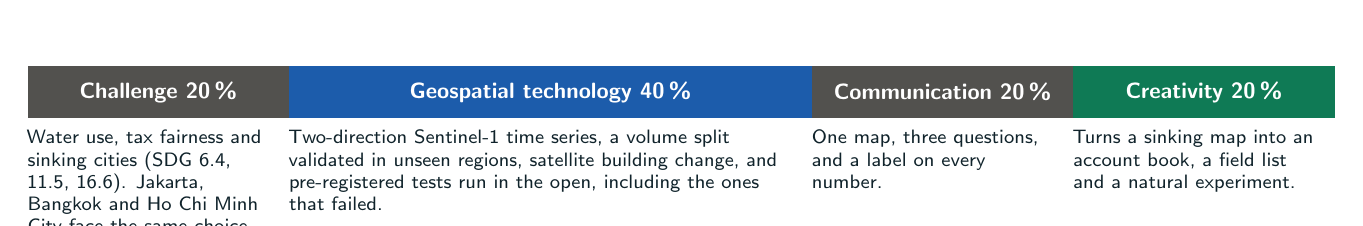
\begin{tikzpicture}[font=\sffamily\scriptsize]
  \tikzset{seg/.style={minimum height=6.5mm,inner sep=0pt,anchor=west,text=white,font=\sffamily\bfseries\fontsize{7.6}{9}\selectfont},
           why/.style={anchor=north west,align=flush left,inner sep=0pt,text=ink}}
  \node[seg,fill=muted,minimum width=33.2mm] (s1) at (0,0) {Challenge 20\,\%};
  \node[seg,fill=accent,minimum width=66.4mm] (s2) at (33.2mm,0) {Geospatial technology 40\,\%};
  \node[seg,fill=muted,minimum width=33.2mm] (s3) at (99.6mm,0) {Communication 20\,\%};
  \node[seg,fill=green,minimum width=33.2mm] (s4) at (132.8mm,0) {Creativity 20\,\%};
  \node[why,text width=30mm] at ($(s1.south west)+(0,-1.5mm)$) {Water use, tax fairness and sinking cities (SDG 6.4, 11.5, 16.6). Jakarta, Bangkok and Ho Chi Minh City face the same choice.};
  \node[why,text width=62mm] at ($(s2.south west)+(0,-1.5mm)$) {Two-direction Sentinel-1 time series, a volume split validated in unseen regions, satellite building change, and pre-registered tests run in the open, including the ones that failed.};
  \node[why,text width=30mm] at ($(s3.south west)+(0,-1.5mm)$) {One map, three questions, and a label on every number.};
  \node[why,text width=30.5mm] at ($(s4.south west)+(0,-1.5mm)$) {Turns a sinking map into an account book, a field list and a natural experiment.};
\end{tikzpicture}
\clearpage
\restoregeometry

\section*{About this document}
\markboth{About this document}{About this document}

This document follows \emph{Groundwater Audit from Space} (the v2 report and its experiments log). That work
asked whether satellites can find and size single pumping wells; the answer for Semarang was no. This
document designs the app that uses what did work. Its research basis is experiment file 15 and files
04--14 of the experiments log \cite{exp15}.

\textbf{Assumptions.} Study area: Central Java for module A, Semarang--Demak for B and C. Team: four
students. Time: six weeks to the national round. Data: only open data and documents a citizen can request.

\subsection*{How to read this document}

Every item that matters has a tag: a letter for its kind and a circled number. For example, \Q{1} (how much
is pumped and paid?) is answered by method \M{1}, checked by \V{1}, built in component \Sx{2}, and
delivered as output \Ox{1}. Section~\ref{sec:trace} lists every link.

\begin{center}
\small\renewcommand{\arraystretch}{1.0}
\begin{tabular}{@{}llp{62mm}l@{}}
\toprule
\textbf{Tag} & \textbf{Kind} & \textbf{Meaning} & \textbf{Defined in}\\*
\midrule
\Q{1}--\Q{3} & Question & What the app must answer & Section~\ref{sec:why}\\
\D{1}--\D{9} & Data & A data set and where it comes from & Section~\ref{sec:data}\\
\M{1}--\M{6} & Method & One step that turns data into an output & Sections~\ref{sec:a}--\ref{sec:c}\\
\V{1}--\V{8} & Validation & A check with a pass mark & Section~\ref{sec:valid}\\
\R{1}--\R{8} & Risk & What could go wrong, and the response & Section~\ref{sec:risks}\\
\U{1}--\U{6} & User need & What a user must be able to do & Section~\ref{sec:product}\\
\Sx{1}--\Sx{6} & Software & A component of the app & Section~\ref{sec:arch}\\
\Ox{1}--\Ox{5} & Output & Something the project delivers & Section~\ref{sec:why}\\
\bottomrule
\end{tabular}
\end{center}

A second kind of label says \emph{what backs a number}. It appears next to every value in the tables and on
every number in the app.

\begin{center}
\small\renewcommand{\arraystretch}{1.05}
\begin{tabular}{@{}lp{110mm}@{}}
\toprule
\textbf{Label} & \textbf{Meaning}\\*
\midrule
\Off & A government regulation, official statistic or official open data set.\\
\Mea & A satellite or field measurement.\\
\Tst & Our own method, which passed a test whose pass mark was fixed before the run.\\
\Calc & Arithmetic on backed inputs. It carries their ranges.\\
\Wk & Only one secondary source (news, blog). Shown, but flagged until confirmed.\\
\Scn & An assumption. The app shows it as a slider the user moves, never as a finding.\\
\Mis & Not obtained yet. The app hides the layer until it is.\\
\bottomrule
\end{tabular}
\end{center}

Three kinds of boxes recur. \textcolor{accent}{\textsf{\textbf{In short}}} gives the point of a
section. \textcolor{green}{\textsf{\textbf{In plain words}}} explains an idea without jargon.
\textcolor{warm}{\textsf{\textbf{Honest limit}}} says what a result does not show.

{\sffamily\footnotesize\hypersetup{linkcolor=ink}\setcounter{tocdepth}{1}\setlength{\parskip}{0pt}\makeatletter\renewcommand*\l@section{\@dottedtocline{1}{0em}{2.2em}}\makeatother\tableofcontents}
\clearpage

\clearpage\part{Research report}
\section{Why this app}\label{sec:why}

\begin{inshort}
The first app idea was a map of every pumping well and its volume. Our own tests ruled that out, and a
plain sinking map already exists online. NERACA moves the question from ``where is each well'' to
\emph{who pumps, who pays, and what to do}, using only results that passed a test or come from official
records.
\end{inshort}

\subsection{What the earlier research settled}\label{sec:found}

Fourteen real-data experiments on Semarang, Arizona and Houston \cite{exp15} leave three facts that shape
this app.

\begin{enumerate}
\item \textbf{Volumes are reliable only at a coarse scale.} A known regional pumping total, split over
  16\,km cells by water demand and sinking volume, landed within about 1.5 times the metered truth in two
  regions it had never seen \cite{exp09}. Finer splits (2--8\,km) failed \cite{exp12}.
\item \textbf{Sinking does not point at wells.} Registered deep wells in Semarang sit on ground that sinks
  \emph{slower} than built-up land of the same density (35.9 vs 48.5\,mm/yr), and sinking bowls lie near
  wells no more often than chance \cite{exp13}.
\item \textbf{Sinking is soft clay times a regional pressure fall.} Clay thickness explains about 80\,\% of
  the pattern; new ground and buildings add about 10\,\%; pumping proxies add nothing beyond that. Heads at
  six observation wells fell in step with sinking. The fastest areas slowed from 113 (2014--17) to 103
  (2018--22) to 89\,mm/yr (2023--26) \cite{exp14}.
\end{enumerate}

\begin{plain}
The satellite can tell how fast the ground sinks, how that changes, and roughly how much water a whole
district pumps. It cannot tell which factory pumps. So the app lets the satellite do the first three, and
lets permits, tariffs and inspectors do the rest.
\end{plain}

Sinking maps and flood projections for Semarang are already published \cite{abidin2013,aditiya2023}, so another sinking map
would not be new. What is missing is a link between the sinking, the water that is pumped, the water that
is declared and paid for, and the piped water that could replace it.

\subsection{Questions and outputs}

\begin{center}
\small
\begin{tabularx}{\linewidth}{@{}L{8mm}Y L{32mm}@{}}
\toprule
 & \textbf{Question} & \textbf{User}\\
\midrule
\Q{1} & How much groundwater is used compared with what is declared, and what is the difference worth in tax? & Tax office (Bapenda), Dinas ESDM, council\\
\Q{2} & Where are new large water users that probably drilled a well without a permit? & Dinas ESDM inspectors\\
\Q{3} & Where does piped water replace the most groundwater, and does sinking slow after it arrives? & PDAM, Bappeda, public works\\
\bottomrule
\end{tabularx}
\end{center}

\begin{center}
\small
\begin{tabularx}{\linewidth}{@{}L{8mm}Y L{24mm}@{}}
\toprule
 & \textbf{Output} & \textbf{Answers}\\
\midrule
\Ox{1} & Groundwater account per regency/city: declared, estimated (range), tariff, tax per 1\Mm & \Q{1}\\
\Ox{2} & Inspection lead list for Semarang--Demak, with a field-feedback record per lead & \Q{2}\\
\Ox{3} & Pipe-priority map with visible, adjustable weights & \Q{3}\\
\Ox{4} & Result of the SPAM Semarang Barat before/after test, with placebos & \Q{3}\\
\Ox{5} & Source register: every number in the app linked to its source and label & all\\
\bottomrule
\end{tabularx}
\end{center}

\subsection{Sustainable Development Goals}

\begin{center}
\small
\begin{tabularx}{\linewidth}{@{}L{22mm}Y@{}}
\toprule
\textbf{Target} & \textbf{How NERACA serves it}\\
\midrule
SDG 6.4 & Water-use efficiency and sustainable withdrawals: accounts (A) and enforcement (B).\\
SDG 6.1 & Safe, affordable drinking water: where piped supply should go next (C).\\
SDG 11.5 & Fewer people affected by disasters: slowing subsidence and tidal flooding (C).\\
SDG 16.6 & Effective, accountable institutions: declared vs estimated use in the open (A, B).\\
SDG 17.1 & Domestic revenue: groundwater tax that is owed but not collected (A).\\
\bottomrule
\end{tabularx}
\end{center}

\subsection{Data}\label{sec:data}

{\small
\begin{xltabular}{\linewidth}{@{}L{8mm}L{44mm}Y L{17mm}@{}}
\caption{Data sets. All are open or can be requested by a citizen.}\label{tab:data}\\*
\toprule
 & \textbf{Data} & \textbf{Source and access} & \textbf{Label}\\*
\midrule
\endfirsthead
\toprule
 & \textbf{Data} & \textbf{Source and access} & \textbf{Label}\\*
\midrule
\endhead
\D{1} & Sentinel-1 ground motion, Semarang 2014--2026 & LiCSAR frames 076D and 127A, already processed \cite{morishita2020,exp14} & \Mea\\
\D{2} & Declared abstraction and NPA per regency/city, 2020--2023 & Dinas ESDM Jateng open data, XLSX, CC-BY \cite{esdmdata,esdmpct} & \Off\\
\D{3} & Groundwater price (NPA) table & Pergub Jateng 7/2025 with annex \cite{pergub7} & \Off\\
\D{4} & Semarang water use, PDAM sales, registered volumes & Perda Kota Semarang 2024 background text \cite{perdasmg} & \Off\\
\D{5} & Built-up change and building footprints & GHSL, Landsat 1988--2024, OSM \cite{ghsl,exp14} & \Mea\\
\D{6} & Groundwater conservation zones, CAT Semarang--Demak & Dinas ESDM Jateng 2022 map under Permen ESDM 31/2018 \cite{undip,idx} & \Off, map to digitise\\
\D{7} & Soft-clay thickness & Boreholes and models, used in \cite{exp14} & \Mea\\
\D{8} & SPAM Semarang Barat capacity, uptake, service area & Government releases \cite{setkab,ekon,investortrust}; service map not yet obtained & \Off\ / \Mis\\
\D{9} & Arizona well registry and metered pumping & ADWR Wells 55 and meters, used in \cite{exp05} & \Off\\
\bottomrule
\end{xltabular}}

\section{A. Groundwater accounts}\label{sec:a}

\begin{inshort}
For each regency and city of Central Java, module A puts three numbers side by side: what was declared,
what our validated method estimates, and what the difference is worth under the official tariff. The
tariff side is fully official. The gap is not known yet, and the app says so with a range.
\end{inshort}

\subsection{Declared use}

Dinas ESDM Jateng publishes the declared abstraction volume and its NPA for every regency and city, as XLSX
files for 2020, 2021, 2022 and 2023 \cite{esdmdata}. Kota Semarang declared 10,069,814\,\mthree\ in 2023 \Off.
A second data set gives use as a share of availability, 2019--2023 \cite{esdmpct}. Module A can therefore
cover all 35 regencies and cities, not only Semarang.

The city's own records show a longer series of registered abstraction \cite{perdasmg}:

\begin{center}
\small
\begin{tabular}{@{}lrrrrrrrr@{}}
\toprule
Year & 1990 & 1995 & 2000 & 2016 & 2017 & 2018 & 2019 & 2023\\
\midrule
Wells & -- & 300 & 320 & 1,050 & -- & -- & -- & --\\
Volume (\Mm) & 23 & 27 & 38 & 13.1 & 15.5 & 27.7 & 13.8 & 10.1\\
\bottomrule
\end{tabular}
\end{center}

\begin{caution}
The series jumps from 13.8 to 27.7\Mm\ between neighbouring years. The declared numbers are themselves
noisy, so a fall from 38 (2000) to 10 (2023) mixes three things: real decline, under-reporting and wells
that were never registered.
\end{caution}

\subsection{Who pumps}

The same document says 96\,\% of registered abstraction is industrial. PDAM (the city water company)
supplied 62\,\% of household demand and distributed 51.66\Mm\ in 2022: 41.63 to households, 4.35 to
commerce and \textbf{only 0.22 to industry} \Off\ \cite{perdasmg}. Industry therefore runs almost entirely
on its own groundwater. The text also says about 19\,\% of supply comes from deep groundwater; the wording
does not make clear whether this is PDAM's own wells.

\subsection{The official price}\label{sec:npa}

Pergub Jateng 7/2025 (in force 18 February 2025) sets the groundwater price, NPA, as \cite{pergub7}:
\[
\text{NPA} = \text{HAB} \times \text{BAT},\qquad \text{BAT} = 0.6\,S + 0.4\,P .
\]
HAB is the base price of water: Rp 2,561 (Wilayah A), 2,795 (B) and 2,824 (C) per \mthree. Wilayah C is
Kota Semarang, Kab.\ Demak, Kab.\ Kudus, Kab.\ Pekalongan and Kota Surakarta. $S$ is the resource
component (16, 9, 4 or 1, by water quality and whether an alternative source exists). $P$ is the use group:
Kelompok 1 sells water as a product, 2--4 are high-, medium- and low-risk businesses, 5 is social,
government and public water supply. Five volume tiers run from 0--50 to more than 2,500\,\mthree. The pages
read do not state the period the tiers refer to.

\begin{table}[H]
\centering\small
\caption{NPA in Wilayah C, good quality with an alternative source (annex table 3a), and the tax at 20\,\%.
All values \Off\ except the tax column \Calc.}\label{tab:npa}
\begin{tabular}{@{}lrrr@{}}
\toprule
\textbf{Use group} & \textbf{NPA, 0--50\,\mthree} & \textbf{NPA, $>$2,500\,\mthree} & \textbf{Tax, top tier}\\
 & Rp/\mthree & Rp/\mthree & Rp/\mthree\\
\midrule
K1 water as a product & 37,277 & 78,575 & 15,715\\
K2 high-risk business & 35,018 & 67,143 & 13,429\\
K3 medium-risk business & 32,758 & 55,701 & 11,140\\
K4 low-risk business & 30,499 & 44,269 & 8,854\\
K5 social, government, public supply & 28,240 & 32,826 & 6,565\\
\bottomrule
\end{tabular}
\end{table}

The annex prints the 40\,\% $P$ column for Wilayah C as 0.40--2.02 for every group, which looks like a typo;
the BAT totals match Wilayah A, so the NPA column is used as printed.

\textbf{Tax rate.} Kota Semarang taxes groundwater (PAT) at 20\,\% of NPA under Perda 10/2023, amended by
Perda 4/2025 \cite{ddtcsmg,perda10}. 20\,\% is also the maximum under UU 1/2022 \cite{terc}. This comes
from a tax news service and a policy brief; the Perda clause itself was not read \Wk.

\textbf{Who is exempt.} Basic household use is reported as exempt, by one secondary source \cite{enforcea}
\Wk. The UU 1/2022 article must be read before households are left out of the rupiah figure.

\subsection{Method \M{1}: declared vs estimated}

The estimate comes from two earlier results:
\begin{itemize}
\item the demand model of file 07 at 4\,km cells, which gives Kota Semarang 25--48\Mmyr\ (median 36.5) but
  was never validated \cite{exp07};
\item the validated split of file 09 at 16\,km, which gives the west and central cell 27.9 / 43.8 /
  54.7\Mmyr\ (P10 / P50 / P90) \cite{exp09} \Tst.
\end{itemize}

The taxable gap is then
\[
\text{gap} = \text{estimated total} - \text{household wells (exempt)} - \text{public supply wells} - \text{declared}.
\]

\begin{table}[htbp]
\centering\small
\caption{The gap for Kota Semarang with today's inputs.}\label{tab:gap}
\begin{tabularx}{\linewidth}{@{}L{48mm}L{26mm}Y l@{}}
\toprule
\textbf{Term} & \textbf{Value, \Mmyr} & \textbf{Basis} & \textbf{Label}\\
\midrule
Estimated total & 25--55 & Files 07 and 09 & \Tst\ / \Calc\\
Household wells outside PDAM & 0--25 & PDAM households $41.63\times38/62$, an upper bound that includes shallow wells and springs & \Calc\\
Public supply wells & 0--10 & About 19\,\% of PDAM supply, if these wells are not already in the declared volume & \Wk\\
Declared (2023) & 10.1 & ESDM open data & \Off\\
\midrule
\textbf{Taxable gap} & \textbf{below 0 to about 45} & Low: $25-25-10-10$; high: $55-0-0-10$ & \Calc\\
\bottomrule
\end{tabularx}
\end{table}

\begin{caution}
With today's inputs we cannot say that there \emph{is} a gap. The household term is the largest unknown.
The app shows this range and the terms that make it up; it does not print a single ``lost revenue''
number. The range narrows when \V{1} is run and when household well use is measured or requested.
\end{caution}

\subsection{Method \M{2}: pricing}

Pricing is plain arithmetic on official numbers: tax per \mthree\ $=0.20\times$ NPA \Calc. For business use in
the top tier (K4 to K2), each 1\Mm\ of undeclared pumping is \textbf{Rp 8.9--13.4 billion per year} in tax.
Pricing the declared 10.07\Mm\ at the K3--K2 top tier gives Rp 112--135 billion per year; this is the
\emph{size} of the tax base, not a measured revenue.

The app shows a slider for ``undeclared business use'' \Scn, starting at zero, and prices whatever the user
sets. Earlier drafts printed a scenario of 5--15\Mm\ (Rp 45--200 billion); this document drops it as a
finding because nothing measured backs it.

\subsection{The first check, \V{1}: billing}\label{sec:v1}

Get the realised groundwater tax for Kota Semarang, 2020--2025, from the budget realisation report (APBD)
or the mayor's accountability report (LKPJ). Divide it by the declared volume of the same year. The
implied price per \mthree\ should fall inside $0.20\times$ the NPA range of groups 2--4.
\begin{itemize}
\item Inside the range: billing matches the declarations; any gap is about undeclared volume.
\item Below the range: tax is leaking at the billing stage, before any unregistered well is counted. This is
  the strongest single number for the pitch, and it needs no satellite data.
\end{itemize}

\begin{caution}
Pergub 7/2025 applies from February 2025. For 2020--2024 the previous NPA regulation applies, and we have
not obtained it yet (\R{1}).
\end{caution}

\section{B. Inspection leads}\label{sec:b}

\begin{inshort}
Module B gives inspectors a short list of places to visit: new large buildings inside zones where no new
well permit can be issued, and outside the reach of piped water. A building like that must get water from
somewhere. Each visit is recorded in the app, which over time builds the per-site record that no open data
set has.
\end{inshort}

\subsection{Why not use sinking to find wells}

The first version of B ranked ``sinking that permits do not explain'' as a hunt for illegal wells. The
experiments made this unsound: sinking follows clay thickness and a regional pressure fall, and registered
wells sit on \emph{slower} ground \cite{exp13,exp14}. Unexplained sinking does not mean an illegal well. B
therefore uses building change and zoning. Sinking appears only as background, to show how damaged a zone
is.

\subsection{Facts that support the leads}

\begin{itemize}
\item \textbf{The zoning exists.} Dinas ESDM Jateng mapped the groundwater conservation zones of the CAT
  Semarang--Demak in 2022 under Permen ESDM 31/2018 \cite{undip,idx} \Off. The ``damaged'' (rusak) zone
  covers most of Kota Semarang. In critical and damaged zones no new abstraction permit can be issued;
  renewals get 50\,\% of the earlier volume and must build recharge wells.
\item \textbf{Industry depends on wells.} PDAM sold 0.22\Mm\ to industry in 2022 \cite{perdasmg} \Off.
\item \textbf{Unregistered wells are common.} In West Java, Dinas ESDM counted at least 6,000 well points,
  of which about 200 had a permit, and is remapping wells to raise tax \cite{ddtcjabar} \Wk. This is
  another province, from a news report.
\item \textbf{Satellites already find unrecorded abstraction elsewhere.} Jordan compared irrigated area from
  Landsat with recorded abstraction and found unlicensed wells and faulty meters \cite{jordan}. In Peru's
  Ica Valley, illicit use was about twice the regulated volume \cite{ica}. EU regulators rate optical and
  radar methods as mature but needing local tuning \cite{impel}.
\end{itemize}

\begin{caution}
All the foreign cases are irrigation, where crops show water use through evaporation. A factory well shows
nothing from space. B relies on a chain of reasoning (new, large, banned zone, no pipes, so probably a well),
and the chain must be tested (\V{4}, \V{5}).
\end{caution}

\subsection{Method \M{3}: the lead filter}

A building becomes a lead when it passes four filters. There is no weighted score: a score with made-up
weights would be a number with nothing behind it.

\begin{center}
\small
\begin{tabularx}{\linewidth}{@{}L{6mm}L{48mm}Y l@{}}
\toprule
 & \textbf{Filter} & \textbf{Data} & \textbf{Label}\\
\midrule
1 & Built after the 2022 zone map & GHSL and Landsat built-up change, building footprints \D{5} & \Mea\\
2 & Footprint above a size threshold, in a water-using class (factory, hotel, mall, hospital) & Footprints, OSM land use \D{5} & \Mea\\
3 & Inside a critical or damaged zone & Zone map \D{6} & \Off\\
4 & Outside the PDAM network & PDAM coverage per village (kelurahan) & \Mis\\
\bottomrule
\end{tabularx}
\end{center}

Filter 4 is the weakest link: the PDAM network map is not public. Until coverage is obtained (a PPID
information request to PDAM or the city), the app uses a proxy: distance to known mains and the SPAM
service districts. Leads based on the proxy are labelled as such.

\subsection{Method \M{4}: the field-feedback loop}

Each lead has a card with a satellite image, footprint, zone and PDAM status, and a button for the
inspector to record what was found:
\emph{registered well / unregistered well / no well / PDAM customer}. The records give two things:
\begin{itemize}
\item the hit rate of B per lead class, measured in the field (\V{6});
\item a growing per-site register, the data that files 12 and 13 showed is missing \cite{exp12,exp13}.
\end{itemize}

Lead cards are for inspectors only. The public view shows counts per district, not addresses: a lead is a
reason to visit, not an accusation (\R{7}).

\subsection{How B is checked}

\begin{itemize}
\item \V{4} \textbf{Arizona retro test.} Arizona registers every well with a drilling date and location
  (Wells 55), already used in file 05 \cite{exp05}. Do new large buildings outside water-provider service
  areas get a new registered well within 500\,m in the same or next two years, more often than
  built-matched random buildings? Pass marks are in Table~\ref{tab:valid}.
\item \V{5} \textbf{Semarang permit overlap.} Leads that fall on a known permitted well (Lo et al.\
  \cite{lo2022} or an ESDM permit list) are confirmed water users. Leads should hit permitted wells more
  often than random new buildings of the same size.
\item \V{6} \textbf{Field hit rate.} Reported per lead class with a 90\,\% interval. It has no pass mark:
  it is the number B exists to measure.
\end{itemize}

\begin{caution}
B cannot measure how many unpermitted wells it misses; that needs a full census. Factories that were already
self-supplied before 2022 are not ``new'' and are not leads. They belong to the declared volume in A.
\end{caution}

\section{C. Pipes instead of pumps}\label{sec:c}

\begin{inshort}
Module C shows where piped surface water would replace the most groundwater, and tests on real data
whether it already slowed the sinking where it arrived. Semarang has a natural experiment: SPAM Semarang
Barat brought about 19\Mmyr\ of reservoir water online in 2022--2024, about twice the city's whole
declared groundwater use.
\end{inshort}

\subsection{Facts}

\begin{itemize}
\item \textbf{SPAM Semarang Barat} is a public--private water project drawing on the Jatibarang reservoir.
  Design capacity is 1,000\,L/s (31.5\Mmyr); uptake was 605\,L/s in January 2024 (about 19\Mmyr) with
  about 44,000 house connections, aiming at 70,000 in Semarang Barat, Tugu and Ngaliyan. The President
  opened it on 23 January 2024 \cite{setkab,ekon,investortrust} \Off.
\item \textbf{Bangkok} combined a groundwater charge, piped-water expansion and a ban on pumping where
  piped supply exists. Subsidence fell to about 0--1\,cm/yr in most areas. The gaps were enforcement and
  household wells, because groundwater was cheaper than piped water \cite{mekong,iges,wbbangkok}.
\item \textbf{Ho Chi Minh City} cut extraction from 716,581 to 252,528\,\mthree/day by the end of 2024,
  aiming at 100,000, by sealing wells \cite{tuoitre} \Wk.
\item \textbf{Jakarta} bans groundwater for large buildings in nine zones and 12 road segments from August
  2023 (Pergub 93/2021). PAM Jaya coverage is reported at 66--82\,\%, with a 100\,\% target by 2030
  \cite{tirto,koranjkt} \Wk.
\end{itemize}

\subsection{Method \M{5}: the pipe-priority map}

Three layers, combined with weights the user can see and move:
\begin{enumerate}
\item groundwater demand not served by PDAM: file 07 at 4\,km (unvalidated, labelled so) and file 09 at
  16\,km \Tst\ \cite{exp07,exp09};
\item damage potential: soft-clay thickness \D{7} \Mea, the main driver of sinking \cite{exp14};
\item planned and new supply: SPAM service districts and other projects \D{8}.
\end{enumerate}

The ranking of places inside a city failed validation in file 12 \cite{exp12}, so the weights are a
\Scn: the map shows what the user's priorities imply, not a prediction.

\subsection{Method \M{6}: did the pipes slow the sinking?}\label{sec:did}

\begin{plain}
Sinking slowed across the whole city after 2018. If piped water helped locally, it should have slowed
\emph{more} where SPAM Semarang Barat connected homes than in similar places it did not reach.
\end{plain}

\textbf{Design.} A difference-in-differences on the Sentinel-1 rate maps already processed \D{1}:
\[
\Delta = (\bar v_{2023\text{--}26} - \bar v_{2018\text{--}22})_{\text{served}} - (\bar v_{2023\text{--}26} - \bar v_{2018\text{--}22})_{\text{matched control}} .
\]
Served cells are in Semarang Barat, Tugu and Ngaliyan; controls are cells elsewhere matched on clay
thickness and built-up share, the two drivers found in file 14 \cite{exp14}. The common slowdown cancels
in the difference.

\textbf{Checks.}
\begin{itemize}
\item \V{7} \textbf{Placebos.} The same test with a fake start (2014--17 vs 2018--22, before the pipes) and
  with fake service areas must show no effect. A shift null (moving the served area at random) gives the
  significance level.
\item \V{8} \textbf{Positive control in Arizona.} Areas where reservoir water replaced metered pumping, so
  the cut is known. The same test must detect it there.
\end{itemize}

\begin{caution}
Test T4 in file 05 already failed: in Arizona, changes in metered pumping did not show up as changes in
sinking \cite{exp05}. So \V{8} may fail too, and C should be ready for that. Three more reasons a real
effect could be hidden: clay keeps compacting for years after pumping stops; the pressure fall is regional,
so local relief spreads over the whole aquifer; and the west has thin clay (about 20\,m), so it sinks
less and has less room to slow.
\end{caution}

\begin{center}
\small
\begin{tabularx}{\linewidth}{@{}L{52mm}Y@{}}
\toprule
\textbf{Outcome} & \textbf{What the app will say}\\
\midrule
\V{7} passes, placebos clean & Sinking slowed more where pipes arrived. Evidence for pipes as a local fix. \\
No extra slowdown, \V{8} passes & The method can see a pumping cut, and saw none here. Pipe priority should follow the volume replaced, not the location.\\
No extra slowdown, \V{8} fails & Inconclusive. The app shows the before/after maps without a claim.\\
Placebo shows an effect & The method picks up noise. No claim.\\
\bottomrule
\end{tabularx}
\end{center}

\textbf{Also unknown:} whether the new customers used groundwater before connecting. If most came from
shallow wells or water vendors, deep pumping did not change and no effect is expected.

\section{What backs each number}\label{sec:backing}

\begin{inshort}
Every number the app shows is listed here with its source and label. A number without a source becomes a
slider (\Scn) or stays hidden (\Mis). Today three inputs are missing and two are weak; the rest is official,
measured or tested.
\end{inshort}

{\small
\begin{xltabular}{\linewidth}{@{}L{52mm}Y l@{}}
\caption{Module A, groundwater accounts.}\label{tab:backa}\\*
\toprule
\textbf{Number on screen} & \textbf{Backed by} & \textbf{Label}\\*
\midrule
Declared volume per regency/city & ESDM Jateng open data 2020--23 \cite{esdmdata}; Semarang series in \cite{perdasmg} & \Off\\
NPA per \mthree & Pergub Jateng 7/2025, annex table 3a \cite{pergub7} & \Off\\
20\,\% tax rate & UU 1/2022 maximum \cite{terc}; Semarang Perda via a tax news service \cite{ddtcsmg} & \Off\ / \Wk\\
Tax per 1\Mm & $0.20\times$ NPA & \Calc\\
Industry runs on its own wells & PDAM sold industry 0.22\Mm\ in 2022 \cite{perdasmg} & \Off\\
Estimated total use, 16\,km & Validated split, file 09 \cite{exp09} & \Tst\\
Estimated total use, 4\,km & Demand model, file 07 \cite{exp07} & \Calc, unvalidated\\
Household exemption & One secondary source \cite{enforcea} & \Wk\\
Household wells outside PDAM & Upper bound from PDAM household sales & \Calc\\
Taxable gap & Table~\ref{tab:gap} & \Calc, wide range\\
Undeclared business use & Set by the user & \Scn\\
Realised groundwater tax & APBD / LKPJ realisation reports & \Mis\\
\bottomrule
\end{xltabular}}

{\small
\begin{xltabular}{\linewidth}{@{}L{52mm}Y l@{}}
\caption{Module B, inspection leads.}\label{tab:backb}\\*
\toprule
\textbf{Number or layer on screen} & \textbf{Backed by} & \textbf{Label}\\*
\midrule
New building and when it appeared & GHSL, Landsat change, footprints, OSM \cite{ghsl,exp14} & \Mea\\
Building class (factory, hotel, \ldots) & OSM land use and tags & \Mea\\
Zone where new wells are banned & ESDM 2022 zone map \cite{undip,idx} & \Off\\
Outside piped water & PDAM coverage per village & \Mis\ (proxy until obtained)\\
Likely to have a well & Industry's PDAM use \cite{perdasmg}; West Java remapping \cite{ddtcjabar} & \Off\ / \Wk\\
Lead hit rate & Field feedback \V{6}; Arizona test \V{4} & \Tst\ once run\\
\bottomrule
\end{xltabular}}

{\small
\begin{xltabular}{\linewidth}{@{}L{52mm}Y l@{}}
\caption{Module C, pipes instead of pumps.}\label{tab:backc}\\*
\toprule
\textbf{Number or layer on screen} & \textbf{Backed by} & \textbf{Label}\\*
\midrule
Sinking rate per period & Sentinel-1 LiCSAR; repeatable across periods and tracks \cite{exp04}; matches ALOS-1 2006--10 \cite{exp10} & \Mea, \Tst\\
Soft-clay thickness & Boreholes; explains about 80\,\% of sinking \cite{exp14} & \Mea, \Tst\\
SPAM Semarang Barat volume & 1,000\,L/s design, 605\,L/s taken up \cite{setkab,ekon} & \Off\\
SPAM service area & Not obtained; districts named in releases used meanwhile & \Mis\\
Pipe-priority weights & Set by the user & \Scn\\
``Pipes slowed the sinking'' & Only after \V{7} and \V{8} & \Tst\ once run\\
\bottomrule
\end{xltabular}}

\section{Validation plan}\label{sec:valid}

\begin{inshort}
Eight checks. Three are done. The other five have pass marks fixed here, before any data are looked at, as
in files 13 and 14. A failure is reported as a failure.
\end{inshort}

{\small
\begin{xltabular}{\linewidth}{@{}L{30mm}Y L{24mm}@{}}
\caption{Validation checks, pass marks and status.}\label{tab:valid}\\*
\toprule
\textbf{Check} & \textbf{Pass mark} & \textbf{Status}\\*
\midrule
\endfirsthead
\toprule
\textbf{Check} & \textbf{Pass mark} & \textbf{Status}\\*
\midrule
\endhead
\V{1} Billing (A) & Realised tax $\div$ declared volume lies within $0.20\times$ the NPA range of groups 2--4 for that year (2025: Rp 6,100--13,429/\mthree). Below the range is reported as a billing leak. & Planned; needs \R{1}\\
\V{2} Volume split (A, C) & Error within 1.5$\times$ on unseen regions at 16\,km & \textbf{Done, passed}: 0.16 and 0.14 \cite{exp09}\\
\V{3} Sinking maps (C) & Signals repeat across periods and tracks above a random null & \textbf{Done, passed}: 58--64\,\% vs 27\,\%; 78\,\% across tracks \cite{exp04}\\
\V{4} Arizona leads (B) & Share of new large buildings with a new registered well within 500\,m in years $t$ to $t{+}2$ is at least 1.5$\times$ the built-matched null, one-sided permutation $p<0.05$ & Planned\\
\V{5} Semarang permits (B) & Leads fall on permitted wells more often than random new buildings of the same size, $p<0.05$ & Planned; needs a permit list\\
\V{6} Field hit rate (B) & No pass mark; reported per lead class with a 90\,\% interval & Starts with the first visits\\
\V{7} SPAM test (C) & $\Delta$ below the 5th percentile of the shift null, and both placebos (fake years, fake areas) between the 5th and 95th percentiles & Planned; data on disk\\
\V{8} Positive control (C) & The same test detects a known, metered pumping cut in Arizona & Planned; file 05 T4 warns it may fail\\
\bottomrule
\end{xltabular}}

The pass marks will be copied into pre-registration files beside the code, as for the earlier experiments,
before \V{4}, \V{5}, \V{7} and \V{8} are run.

\section{Risks}\label{sec:risks}

{\small
\begin{xltabular}{\linewidth}{@{}L{8mm}L{50mm}Y@{}}
\caption{Risks and responses.}\label{tab:risks}\\*
\toprule
 & \textbf{Risk} & \textbf{Response}\\*
\midrule
\endfirsthead
\toprule
 & \textbf{Risk} & \textbf{Response}\\*
\midrule
\endhead
\R{1} & The NPA regulation before 2025 is not found, so \V{1} has no price for 2020--2024 & Search the provincial legal database (JDIH); otherwise run \V{1} on 2025 alone\\
\R{2} & Households are not exempt after all & Read the UU 1/2022 article; move household wells into the taxable terms of Table~\ref{tab:gap}\\
\R{3} & PDAM does not release coverage per village & Use the labelled proxy; file a PPID request early\\
\R{4} & The SPAM service area is not available & Use the three named districts as the served area; the test becomes coarser\\
\R{5} & Arizona does not transfer to an Indonesian city & \V{4} checks the logic only; Semarang is judged by \V{5} and \V{6}\\
\R{6} & C finds no effect because of delay or the regional pressure fall & Report it with the outcome table in Section~\ref{sec:did}; no claim either way\\
\R{7} & A lead is read as an accusation against a named company & Lead cards for inspectors only; the public sees district counts\\
\R{8} & Challenge dates or rules differ from the ones listed & Confirm on the official page before planning the final weeks\\
\bottomrule
\end{xltabular}}

\clearpage\part{App design}
\section{The product in brief}\label{sec:product}

\begin{inshort}
NERACA is a static web map with three tabs (Accounts, Leads, Pipes) and one small server piece, the
field-feedback form. Every number has a coloured label; clicking it opens its source.
\end{inshort}

\subsection{Users and what they need}

{\small
\begin{xltabular}{\linewidth}{@{}L{40mm}Y@{}}
\toprule
\textbf{User} & \textbf{Question they bring}\\*
\midrule
Regional tax office (Bapenda) & ``Does the groundwater tax we collect match the water that is used?''\\
Groundwater inspector (Dinas ESDM) & ``Which sites should my team visit this month?''\\
Planner (PDAM, Bappeda, public works) & ``Where should the next piped-water project go, and did the last one help?''\\
Jury and public & ``What does this show, and why should I trust the numbers?''\\
\bottomrule
\end{xltabular}}

{\small
\begin{xltabular}{\linewidth}{@{}L{8mm}Y L{16mm}L{21mm}@{}}
\caption{User needs, with the outputs and components that serve them.}\label{tab:needs}\\*
\toprule
 & \textbf{Need} & \textbf{Output} & \textbf{Component}\\*
\midrule
\U{1} & See declared vs estimated use per regency/city, with ranges and labels. & \Ox{1} & \Sx{2} \Sx{5}\\
\U{2} & Move the ``undeclared business use'' slider and see the tax it implies. & \Ox{1} & \Sx{5}\\
\U{3} & Open the lead list and a lead card: image, footprint, zone, PDAM status. & \Ox{2} & \Sx{3} \Sx{5}\\
\U{4} & Record the outcome of a field visit. & \Ox{2} & \Sx{6}\\
\U{5} & Change pipe-priority weights; read the SPAM before/after result. & \Ox{3} \Ox{4} & \Sx{1} \Sx{5}\\
\U{6} & Click any number and see its source and label. & \Ox{5} & \Sx{5}\\
\bottomrule
\end{xltabular}}

\subsection{Screens}

\begin{enumerate}
\item \textbf{Accounts.} A Central Java map coloured by declared volume per regency/city. A side panel
  shows declared, estimated range, tariff, tax per 1\Mm, and the slider. Each value has its label.
\item \textbf{Leads.} The Semarang--Demak map with zones, PDAM coverage (or its proxy) and lead points.
  A lead card opens on click, with the feedback buttons for signed-in inspectors.
\item \textbf{Pipes.} The pipe-priority map with weight sliders, the sinking maps for 2018--22 and
  2023--26, and the result card of the SPAM Semarang Barat test, worded by the outcome table in
  Section~\ref{sec:did}.
\end{enumerate}

\begin{figure}[H]
\centering
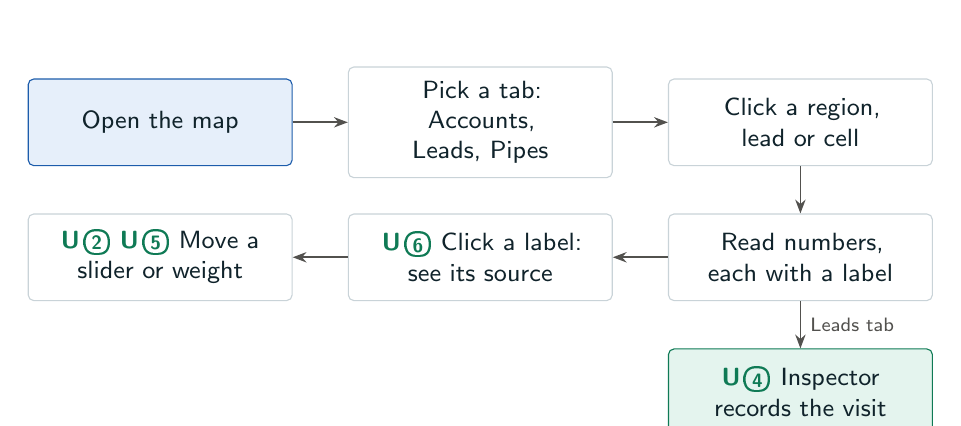
\begin{tikzpicture}[node distance=6mm and 7mm]
\tikzset{uf/.style={box,text width=30mm,minimum height=11mm}}
\node[uf,boxa] (a) {Open the map};
\node[uf,right=of a] (b) {Pick a tab:\\Accounts, Leads, Pipes};
\node[uf,right=of b] (c) {Click a region,\\lead or cell};
\node[uf,below=of c] (d) {Read numbers,\\each with a label};
\node[uf,left=of d] (e) {\U{6} Click a label:\\see its source};
\node[uf,left=of e] (f) {\U{2} \U{5} Move a\\slider or weight};
\node[uf,boxg,below=of d] (g) {\U{4} Inspector\\records the visit};
\draw[arr] (a)--(b); \draw[arr] (b)--(c); \draw[arr] (c)--(d);
\draw[arr] (d)--(e); \draw[arr] (e)--(f);
\draw[arr] (d)-- node[lab,right]{Leads tab} (g);
\end{tikzpicture}
\caption{User flow.}
\end{figure}

\section{Architecture}\label{sec:arch}

\begin{inshort}
The heavy work runs offline in the Python code that already exists. The app itself is static files plus
one form, so it can be hosted for free and still work during judging.
\end{inshort}

\begin{figure}[H]
\centering
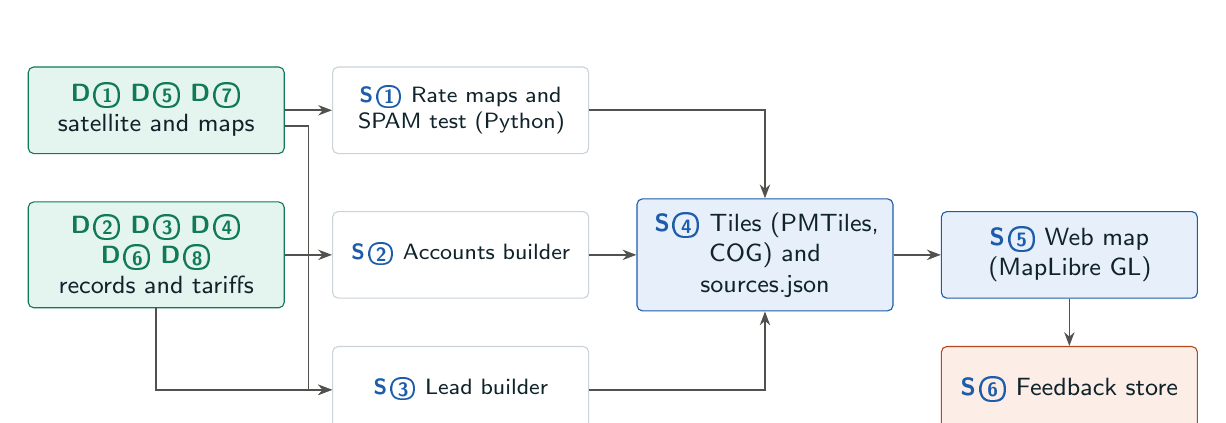
\begin{tikzpicture}[node distance=6mm and 6mm]
\tikzset{cmp/.style={box,text width=29mm,minimum height=11mm,font=\sffamily\footnotesize}}
\node[cmp,boxg] (d1) {\D{1} \D{5} \D{7}\\satellite and maps};
\node[cmp,boxg,below=of d1] (d2) {\D{2} \D{3} \D{4} \D{6} \D{8}\\records and tariffs};
\node[cmp,right=of d1] (s1) {\Sx{1} Rate maps and\\SPAM test (Python)};
\node[cmp,right=of d2] (s2) {\Sx{2} Accounts builder};
\node[cmp,below=of s2] (s3) {\Sx{3} Lead builder};
\node[cmp,boxa,right=of s2] (s4) {\Sx{4} Tiles (PMTiles,\\COG) and sources.json};
\node[cmp,boxa,right=of s4] (s5) {\Sx{5} Web map\\(MapLibre GL)};
\node[cmp,boxw,below=of s5] (s6) {\Sx{6} Feedback store};
\draw[arr] (d1)--(s1); \draw[arr] (d2)--(s2); \draw[arr] (d2.south) |- (s3.west);
\draw[arr] (d1.east) ++(0,-2mm) -- ++(3mm,0) |- (s3.west);
\draw[arr] (s1.east) -| (s4.north); \draw[arr] (s2)--(s4); \draw[arr] (s3.east) -| (s4.south);
\draw[arr] (s4)--(s5); \draw[arr] (s5)--(s6);
\end{tikzpicture}
\caption{Components. Green: data; white: offline Python; blue: static files served to the browser;
orange: the only server piece.}
\end{figure}

{\small
\begin{xltabular}{\linewidth}{@{}L{8mm}L{36mm}Y@{}}
\caption{Software components.}\label{tab:sw}\\*
\toprule
 & \textbf{Component} & \textbf{What it does}\\*
\midrule
\Sx{1} & Rate maps and SPAM test & Existing LiCSAR processing and the cause-test code of file 14; adds the difference-in-differences of \M{6} with placebos.\\
\Sx{2} & Accounts builder & Reads the ESDM XLSX files and the NPA table; joins the 16\,km estimates; writes one record per regency/city with ranges and labels.\\
\Sx{3} & Lead builder & Built-up change, footprints, zone and coverage layers; applies the four filters of \M{3}.\\
\Sx{4} & Tiles and source register & Writes vector tiles (PMTiles), rasters (Cloud-Optimised GeoTIFF) and \texttt{sources.json}, which gives every number its source, link and label.\\
\Sx{5} & Web map & MapLibre GL, three tabs, sliders, lead cards, label badges. No backend.\\
\Sx{6} & Feedback store & One shared table: lead id, inspector, date, outcome, note. Sign-in for inspectors only.\\
\bottomrule
\end{xltabular}}

One entry of the source register:
\begin{verbatim}
{ "id": "npa_C_K2_top", "value": 67143, "unit": "Rp/m3",
  "label": "OFFICIAL",
  "source": "Pergub Jateng 7/2025, annex table 3a",
  "url": "https://peraturan.bpk.go.id/Details/314690/..." }
\end{verbatim}

\section{Beyond Semarang}\label{sec:asean}

\begin{center}
\small
\begin{tabularx}{\linewidth}{@{}L{30mm}L{30mm}L{34mm}Y@{}}
\toprule
\textbf{Place} & \textbf{Sinking data} & \textbf{Declared use} & \textbf{Policy hook}\\
\midrule
Central Java (35) & LiCSAR, Semarang processed & ESDM open data 2020--23 & Pergub 7/2025 tariff, 2022 zones\\
Jakarta & LiCSAR, free & not found yet & Groundwater-free zones, PAM Jaya coverage\\
Ho Chi Minh City & LiCSAR, free & city totals in the news & Well sealing by SAWACO\\
Bangkok & LiCSAR, free & DGR, not checked & Groundwater charge: the success case\\
Manila & LiCSAR, free & nothing found & not checked\\
\bottomrule
\end{tabularx}
\end{center}

The first version covers Central Java fully for A, and Semarang--Demak for B and C. Other cities appear in A
only where official totals exist.

\section{Challenge fit}\label{sec:fit}

The ASEAN Geospatial Challenge is run with the Singapore Land Authority; BIG runs the Indonesian round
\cite{aseangeo,sla}. The theme is the SDGs. Judging weights are Challenge 20\,\%, Geospatial Technology
40\,\%, Communication 20\,\% and Creativity 20\,\%. The listed timeline (registration 4 August to 12
January, judging 26 January, finals 11 February) must be confirmed on the official page (\R{8}).

Geospatial technology is 40\,\% of the score, so the pitch leads with the satellite work: two-direction
Sentinel-1 time series, the validated 16\,km volume split, building change from GHSL and Landsat, and the
pre-registered tests. The tariff and the tax are what make it matter to a government user.

\section{Plan}\label{sec:plan}

{\small
\begin{xltabular}{\linewidth}{@{}L{12mm}Y L{24mm}@{}}
\caption{Six-week plan.}\label{tab:plan}\\*
\toprule
\textbf{Week} & \textbf{Work} & \textbf{Closes}\\*
\midrule
1 & Request realised groundwater tax 2020--25 and the pre-2025 NPA regulation; download the ESDM XLSX files; read the UU 1/2022 exemption and the Semarang Perda; file PPID requests for PDAM coverage and the SPAM service area & \V{1}, \R{1}--\R{4}\\
2 & Write pre-registrations for \V{4}, \V{5}, \V{7}, \V{8}; run \V{7} on the rate maps on disk; digitise the 2022 zone map & \V{7}, \D{6}\\
3 & Run \V{4} and \V{8} in Arizona; build the lead filter & \V{4}, \V{8}, \Sx{3}\\
4 & App skeleton: tiles, Accounts tab, source register & \Sx{2}, \Sx{4}, \Sx{5}\\
5 & Leads and Pipes tabs, feedback form & \Sx{5}, \Sx{6}\\
6 & Results into the app wording; pitch video; write-up & all\\
\bottomrule
\end{xltabular}}

\clearpage\part{Traceability and references}
\Needspace{24\baselineskip}
\section{Traceability}\label{sec:trace}

\begin{inshort}
Read a row from left to right to follow one thread: from a question, through the data and method that
answer it, to the check that tests it, the software that runs it and the output that delivers it.
\end{inshort}

{\small
\begin{xltabular}{\linewidth}{@{}L{24mm}L{22mm}L{16mm}L{22mm}L{20mm}Y@{}}
\caption{From question to output.}\label{tab:traceq}\\*
\toprule
\textbf{Question} & \textbf{Data} & \textbf{Method} & \textbf{Validation} & \textbf{Software} & \textbf{Output}\\*
\midrule
\Q{1} Used, declared, paid? & \D{1} \D{2} \D{3} \D{4} & \M{1} \M{2} & \V{1} \V{2} & \Sx{2} \Sx{4} \Sx{5} & \Ox{1} \Ox{5}\\
\Q{2} Where are new wells? & \D{4} \D{5} \D{6} \D{9} & \M{3} \M{4} & \V{4} \V{5} \V{6} & \Sx{3} \Sx{5} \Sx{6} & \Ox{2} \Ox{5}\\
\Q{3} Do pipes help? & \D{1} \D{7} \D{8} \D{9} & \M{5} \M{6} & \V{2} \V{3} \V{7} \V{8} & \Sx{1} \Sx{4} \Sx{5} & \Ox{3} \Ox{4} \Ox{5}\\
\bottomrule
\end{xltabular}}

{\small
\begin{xltabular}{\linewidth}{@{}L{46mm}L{24mm}L{22mm}L{18mm}Y@{}}
\caption{Each method with its data, checks, software and risks.}\label{tab:tracem}\\*
\toprule
\textbf{Method} & \textbf{Data} & \textbf{Checked by} & \textbf{Runs in} & \textbf{Risks}\\*
\midrule
\M{1} Declared vs estimated & \D{1} \D{2} \D{4} & \V{1} \V{2} & \Sx{2} & \R{2}\\
\M{2} Pricing & \D{3} & \V{1} & \Sx{2} & \R{1}\\
\M{3} Lead filter & \D{5} \D{6} & \V{4} \V{5} & \Sx{3} & \R{3} \R{5} \R{7}\\
\M{4} Field feedback & from \M{3} & \V{6} & \Sx{6} & \R{7}\\
\M{5} Pipe-priority map & \D{1} \D{7} \D{8} & \V{2} \V{3} & \Sx{1} \Sx{5} & \R{4}\\
\M{6} SPAM before/after test & \D{1} \D{7} \D{8} \D{9} & \V{7} \V{8} & \Sx{1} & \R{4} \R{6}\\
\bottomrule
\end{xltabular}}

User needs \U{1}--\U{6} are traced to outputs and components in Table~\ref{tab:needs}.

\section{Glossary}

\begin{description}[leftmargin=34mm,style=nextline,font=\sffamily\bfseries\small,itemsep=1pt]
\item[NPA] Nilai Perolehan Air: the official value of groundwater per \mthree, set by the province. The tax is a share of it.
\item[PAT] Pajak Air Tanah: the regional groundwater tax, collected by the city or regency.
\item[HAB / BAT] Base price of water / the weighting factor for resource and use group. NPA $=$ HAB $\times$ BAT.
\item[CAT] Cekungan Air Tanah: a groundwater basin. CAT Semarang--Demak is zoned as safe, vulnerable, critical or damaged.
\item[PDAM] The city water company. In Semarang: PDAM Tirta Moedal.
\item[SPAM] Sistem Penyediaan Air Minum: a drinking-water supply system, such as SPAM Semarang Barat.
\item[PPID] The public information office that answers citizens' data requests.
\item[APBD / LKPJ] The regional budget / the head of region's annual accountability report; both list realised tax.
\item[InSAR] Measuring ground motion by comparing radar images taken at different times.
\item[Difference-in-differences] Comparing the change in a treated area with the change in similar untreated areas, so that changes common to both cancel.
\item[Placebo test] The same test run where there should be no effect (wrong years, wrong places). If it finds one, the method is picking up noise.
\item[Pre-registration] Writing down the test and its pass mark before looking at the result.
\end{description}

\begin{thebibliography}{99}\small\raggedright
\bibitem{abidin2013} H.Z. Abidin, H. Andreas, I. Gumilar, T.P. Sidiq, Y. Fukuda. Land subsidence in coastal city of Semarang (Indonesia): characteristics, impacts and causes. \emph{Geomatics, Natural Hazards and Risk} 4(3), 226--240, 2013.
\bibitem{aditiya2023} A. Aditiya, T. Ito. Present-day land subsidence over Semarang revealed by time series InSAR new small baseline subset technique. \emph{Int.\ J.\ Applied Earth Observation and Geoinformation} 125, 103579, 2023.
\bibitem{aseangeo} ASEAN Geospatial Challenge. \url{https://www.aseangeospatial.org/asean-geospatial-challenge/}
\bibitem{ddtcjabar} DDTC News. Demi kejar pajak, Dinas ESDM petakan ulang sumur air tanah di daerah, January 2025. \url{https://news.ddtc.co.id/berita/daerah/1808556/demi-kejar-pajak-dinas-esdm-petakan-ulang-sumur-air-tanah-di-daerah}
\bibitem{ddtcsmg} DDTC News. Ketentuan terbaru tarif pajak daerah di Kota Semarang. \url{https://news.ddtc.co.id/berita/daerah/1800913/ketentuan-terbaru-tarif-pajak-daerah-di-kota-semarang-cek-di-sini}
\bibitem{ekon} Kemenko Perekonomian. Pemerintah dorong peningkatan ketersediaan air minum dengan operasional PSN SPAM Semarang Barat. \url{https://ekon.go.id/unduh/publikasi/4380/pemerintah-dorong-peningkatan-ketersediaan-air-minum-dengan-operasional-psn-spam-semarang-barat}
\bibitem{enforcea} Enforcea. Apa itu pajak air tanah. \url{https://enforcea.com/Blog/apa-itu-pajak-air-tanah}
\bibitem{esdmdata} Dinas ESDM Provinsi Jawa Tengah. Nilai Perolehan Air Tanah (NPA) dan volume pengambilan pengusahaan air tanah di Provinsi Jawa Tengah, 2020--2023. \url{https://data.jatengprov.go.id/dataset/fcc-nilai-perolehan-air-tanah-npa-dan-volume-pengambilan-pengusahaan-air-tanah-di-provinsi-jawa-teng}
\bibitem{esdmpct} Dinas ESDM Provinsi Jawa Tengah. Persentase pengambilan air tanah di Jawa Tengah. \url{https://data.jatengprov.go.id/dataset/29a-persentase-pengambilan-air-tanah-di-jawa-tengah}
\bibitem{exp04} Experiments log, file 04: blind test and repeatability. \texttt{docs/groundwater-audit-latex-v2/experiments/04-blind-and-repeatability.md}
\bibitem{exp05} Experiments log, file 05: Arizona metered-pumping validation T1--T7. \texttt{.../experiments/05-arizona-validation.md}
\bibitem{exp07} Experiments log, file 07: Semarang water-demand model. \texttt{.../experiments/07-semarang-demand-model.md}
\bibitem{exp09} Experiments log, file 09: known total split by demand and sinking, validated. \texttt{.../experiments/09-validated-regional-split.md}
\bibitem{exp10} Experiments log, file 10: ALOS-1 PALSAR 2006--2010. \texttt{.../experiments/10-alos1-2006-2010.md}
\bibitem{exp12} Experiments log, file 12: relative heatmap inside a region. \texttt{.../experiments/12-relative-heatmap.md}
\bibitem{exp13} Experiments log, file 13: registered wells vs sinking, pre-registered. \texttt{.../experiments/13-registered-wells-test.md}
\bibitem{exp14} Experiments log, file 14: what explains the sinking. \texttt{.../experiments/14-subsidence-causes.md}
\bibitem{exp15} Experiments log, file 15: app pivot research A+B+C. \texttt{.../experiments/15-app-pivot-a-b-c.md}
\bibitem{ghsl} European Commission Joint Research Centre. Global Human Settlement Layer (GHSL), built-up surface. \url{https://human-settlement.emergency.copernicus.eu/}
\bibitem{ica} Illicit groundwater use in the Ica Valley, Peru. EGU General Assembly 2024, EGU24-11957. \url{https://meetingorganizer.copernicus.org/EGU24/EGU24-11957.html}
\bibitem{idx} IDX Channel. ESDM beberkan wilayah yang cekungan air tanahnya rusak. \url{https://www.idxchannel.com/news/esdm-beberkan-wilayah-yang-cekungan-air-tanahnya-rusak-simak-lokasinya/all}
\bibitem{iges} IGES. Groundwater management in Asian cities, ISAP 2009. \url{https://isap.iges.or.jp/2009/jp/pdf/day2/27m_304asiancities.pdf}
\bibitem{impel} IMPEL. Water Over-abstraction and Illegal Abstraction (WODA), final report, 2015. \url{https://impel.eu/contents/libraryfile/FR-2015-11%20WODA%20Final%20Report.pdf}
\bibitem{investortrust} Investortrust. Kemenkeu ungkap infrastruktur layanan air minum butuh investasi Rp 123,5 triliun. \url{https://investortrust.id/business/34175/kemenkeu-ungkap-infrastruktur-layanan-air-minum-butuh-investasi-rp-123-5-triliun}
\bibitem{jordan} Remote sensing of irrigated area vs recorded groundwater abstraction in Jordan. \url{https://bvbvf1.bib-bvb.de/vufind/PrimoRecord/cdi_proquest_journals_2713850785}
\bibitem{koranjkt} Koran Jakarta. Gubernur DKI Jakarta berkomitmen kejar target cakupan air bersih 100 persen, 30 September 2025. \url{https://koran-jakarta.com/2025-09-30/gubernur-dki-jakarta-berkomitmen-kejar-target-cakupan-air-bersih-100-persen/amp}
\bibitem{lo2022} W. Lo, S.N. Purnomo, B.G. Dewanto, D. Sarah, Sumiyanto. Integration of numerical models and InSAR techniques to assess land subsidence due to excessive groundwater abstraction in the coastal and lowland regions of Semarang City. \emph{Water} 14(2), 201, 2022.
\bibitem{mekong} Mekong--U.S.\ Partnership. How Bangkok stopped sinking, and what the Mekong delta could learn, 2 October 2020. \url{https://mekonguspartnership.org/2020/10/02/how-bangkok-stopped-sinking-and-what-the-mekong-delta-could-learn-october-2-2020/}
\bibitem{morishita2020} Y. Morishita, M. Lazecky, T.J. Wright, J.R. Weiss, J.R. Elliott, A. Hooper. LiCSBAS: an open-source InSAR time series analysis package integrated with the LiCSAR automated Sentinel-1 InSAR processor. \emph{Remote Sensing} 12(3), 424, 2020.
\bibitem{perda10} Perda Kota Semarang No.\ 10 Tahun 2023 tentang Pajak Daerah dan Retribusi Daerah. \url{https://pasal.id/peraturan/perda/perda-kota-semarang-no-10-tahun-2023}
\bibitem{perdasmg} Perda Kota Semarang 2024, background text on water supply and groundwater use (local copy \texttt{realdata/semarang/perda/p.txt}).
\bibitem{pergub7} Peraturan Gubernur Jawa Tengah No.\ 7 Tahun 2025 tentang Penetapan Nilai Perolehan Air Tanah, with annex. \url{https://peraturan.bpk.go.id/Details/314690/pergub-prov-jawa-tengah-no-7-tahun-2025}
\bibitem{setkab} Sekretariat Kabinet. Resmikan SPAM Semarang Barat, Presiden bantu masyarakat peroleh air bersih terjangkau, January 2024. \url{https://setkab.go.id/resmikan-spam-semarang-barat-presiden-bantu-masyarakat-peroleh-air-bersih-terjangkau/}
\bibitem{sla} Singapore Land Authority. ASEAN Geospatial Challenge. \url{https://geospatial.sla.gov.sg/geoworks/asean-geospatial-challenge/}
\bibitem{terc} TERC LPEM FEB UI. Pajak air permukaan dan pajak air tanah, policy brief, 2024. \url{https://terc.lpem.org/wp-content/uploads/2024/04/PAP_dan_PAT-TERC_Brief.pdf}
\bibitem{tirto} tirto.id. Gedung di zona bebas air tanah wajib pakai air PAM Jaya. \url{https://tirto.id/gedung-di-zona-bebas-air-tanah-wajib-pakai-air-pam-jaya-g5dF}
\bibitem{tuoitre} Tuoi Tre News. Ho Chi Minh City reduces groundwater extraction to fight land subsidence. \url{https://news.tuoitre.vn/ho-chi-minh-city-reduces-groundwater-extraction-to-fight-land-subsidence-10325091712283531.htm}
\bibitem{undip} Universitas Diponegoro thesis, chapter 1: CAT Semarang--Demak conservation zones and permit rules. \url{https://eprints2.undip.ac.id/55333/3/Bab%20I.pdf}
\bibitem{wbbangkok} World Bank GW-MATE. Bangkok groundwater management case profile. \url{https://documents1.worldbank.org/curated/en/750761468304831965/pdf/518250BRI0Box31GWMATE1CP1201Bangkok.pdf}
\end{thebibliography}

\end{document}
